%#############################################################
% Autor: Prof. Dr. Kai Luppa
% Fachhochschule Dortmund Fachbereich Informations- und Elektrotechnik
% Stand: Version2.0, 16.11.2017
%
% Dies ist eine Vorlage für Abschlussarbeiten (Bachelor Thesis, Betriebliche Praxis, 
% Projektarbeiten, etc.) Der Dokumentenaufbau (Titelblatt sowie Reihenfolge
% der Verzeichnisse und Anhänge) sollte nicht verändert werden.
%
% In der Päambel sind ggf. BibTex-Datei und die verwendeten Abkürzungen
% anzupassen (beides direkt vor \begin{document}). Im Dokument werden
% Formatierungsvorlagen angewendet, die so als Grundlage von Abschlussarbeiten 
% im Labor für Energieautomatisierung verwendet werden sollten. 
%
% Das Prozentzeichen bedeutet übrigens den Beginn eines Kommentars ;-)
%
% Zum Übersetzen in das PDF-Format die folgenden Aufrufe starten: 
% pdflatex _LaTeX_Vorlage_FHDO_V2.tex
% bibtex _LaTeX_Vorlage_FHDO_V2
% pdflatex _LaTeX_Vorlage_FHDO_V2.tex
% pdflatex _LaTeX_Vorlage_FHDO_V2.tex


%#############################################################
% Hier beginnt die Präambel
\documentclass[a4paper,11pt,ngerman,headsepline,bibtotoc,liststotoc,numbers=noenddot]{scrreprt}

\usepackage[T1]{fontenc}
\usepackage[utf8]{inputenc}
\usepackage[ngerman]{babel}
\usepackage{footmisc} % für Fußnotenreferenzen mit \footref{}
\usepackage[printonlyused]{acronym} % für das Abkürzungsverzeichnis
\usepackage{graphicx} % für die Abbildungen
\usepackage{float} % für die Gleitumgebung (Abbildungen, Tabellen, Listings)
\usepackage{listings} % für die Listings
\usepackage{color} % für grauen Hintergrund der Listings
\usepackage[sorting=nty,backend=bibtex8]{biblatex} % für das Literaturverzeichnis
\usepackage[colorlinks=false]{hyperref} % PDF-Inhaltsverzeichnis und Links einschalten, wird nicht gedruckt
\usepackage{array} % für die zentrierten Spalten mit vorgegebener Breite in einer Tabelle (longtable)
\usepackage[acronym,nomain,nonumberlist,toc]{glossaries} % für die Abkürzungsliste
\usepackage{pdfpages} % zum Einbinden von PDF-Dokumenten
\usepackage{chngcntr} % für durchgängige Fussnotenzählung
%\usepackage{codestyle}


\usepackage[left=2.5cm, right=2.5cm, top=2.5cm, bottom=2.5cm]{geometry}

\counterwithout{footnote}{chapter} % durchgängige Fussnotenzählung

\DefineBibliographyStrings{ngerman}{bibliography = {Literaturverzeichnis}} % Titel für Literatur ändern


\definecolor{grey}{rgb}{0.95,0.95,0.95} % definiere grau für Hintergrund der Listings

% Einstellungen für Listings
%\lstset{captionpos=b, 
%	language=java, 
%	alsolanguage=php,
%	alsolanguage=c,
%	numbers=left,
%	breaklines=true,
%	tabsize=3, 
%	basicstyle=\ttfamily\small,
%	backgroundcolor=\color{grey},
%	numberstyle=\scriptsize, 
%	frame=single, 
%	framerule=0.1pt,
%	showstringspaces=false,
%}

\setcounter{secnumdepth}{3} % drei Abschnitts-Gliederungstiefen
\setcounter{tocdepth}{3} % drei Abschnittsgliederungstiefen im Inhaltsverzeichnis anzeigen

\setlength{\parindent}{0mm} % Länge des Einzungs beim Absatz -> 0mm: kein Einzug
\setlength{\parskip}{0cm} % Vertikale Abstand zu einem neuen Absatz


\renewcommand{\lstlistlistingname}{Quelltextverzeichnis}% Änderung von Listings nach Quelltextverzeichnis
\renewcommand{\lstlistingname}{Quelltext} % Änderung von Listing nach Quelltext
\renewcommand{\arraystretch}{1.2} % Tabellenzeilenabstand um Faktor 1.2 vergrößern
\newcolumntype{C}[1]{>{\centering\arraybackslash}p{#1}} % zentrierte Spalten mit Breitenangabe 
\newcolumntype{R}[1]{>{\raggedleft\arraybackslash}p{#1}} % rechtsbündig mit Breitenangabe 
\newcolumntype{L}[1]{>{\raggedright\arraybackslash}p{#1}} % linksbündig mit Breitenangabe 
\renewcommand*{\glspostdescription}{} % Den Punkt am Ende jeder Beschreibung deaktivieren

\newcommand{\afzsm}[1]{\dq #1\dq}
\newcommand{\afzde}[1]{\glqq #1\grqq}
\newcommand{\afzfr}[1]{\flqq #1\frqq}

\sloppy % Immer im Blocksatz bleiben

\makeglossaries % erstelle die Glossaries, hier nur das Abkürzungsverzeichnis


%**********************************************************************************
% In der Präamble sind nur die folgenden zwei Punkte 
% 1. ggf. BibTex-Datei
% 2. Verwendete Abkürzungen 
% anzupassen

%----------------------------------------------------------------------
% Hier ggf. die BibTex-Datei anpassen (wenn anderer Dateiname gewählt wurde) 

\bibliography{Literatur} % verwende die Datei Literatur.bib im selben Verzeichnis

%----------------------------------------------------------------------
% Hier die Abkürzungsliste bearbeiten 
\newacronym{ac:tcpip}{TCP/IP}{Transmission Control Protocol / Internet Protocol}

%\newacronym{xyz}{XYZ}{lXXX YYY ZZZ}

\newacronym{ac:LED}{LED}{Light Emitting Diode}
\newacronym{ac:tia}{TIA}{Totally Integrated Automation}



\newcommand{\ptitel}{\emph{Betriebliche Praxis}}
\newcommand{\paufgabe}{\emph{Bericht über die Erstellung der Benutzeroberfläche der SIEMENS Comfort Pannels im SIEMENS TIA-Portal}}
\newcommand{\absatz}{\\[0.2cm]}
%---------------------------------------------------------------------
% Hier Definition von eingegebenen Quellcode
 \definecolor{darkgreen}{rgb}{0.0, 0.42, 0.24}
\definecolor{blue-violet}{rgb}{0.55, 0.0, 0.55}
%\lstset{
%	language=python, 				% Setzt die Sprache
%	basicstyle=\scriptsize\ttfamily, 	% Setzt den Standardstil
%	keywordstyle=\color{blue-violet}\bfseries,	% Setzt den Stil für Schlüsselwörter
%	identifierstyle=\color{blue},		% Identifier bekommen keine gesonderte formatierung
%	commentstyle=\color{darkgreen},		% Stil für Kommentare
%	stringstyle=\ttfamily, 			% Stil für Strings (gekennzeichnet mit "String")
%	breaklines=true, 			% Zeilen werden umgebrochen
%	numbers=left, 				% Zeilennummern links
%	numberstyle=\tiny, 			% Stil für die Seitennummern
%	frame=single, 				% Rahmen
%	backgroundcolor=\color{white}, 	% Hintergrundfarbe
%	caption={Python-Code}, 			% Caption
%	tabsize=4				% Größe der Tabulatoren
%}

%#############################################################
% Hier beginnt das Dokument
\begin{document}

%----------------------------------------------------------------------
% Titelseite
\begin{titlepage}
\titlehead{\flushleft
\includegraphics[width=1.0\linewidth]{./_bilder/__fhdologo.png}}%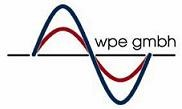
\includegraphics[width=3.64cm,height=2.18cm]{./_bilder/wpe.png}}

\subject{
	Betriebliche Praxis
} 
\title{
	Bericht über die Erstellung der Benutzeroberfläche der SIEMENS Comfort Pannels im SIEMENS TIA-Portal
}
\author{	
	%Aron von dem Berge\\ 
	%\small{Matrikelnummer 7201810}\\
	Frederik Rath\\ 
	\small{Matrikelnummer 7202624}\\
	%Lorena Sträßer\\ % hier den Namen anpassen
	%\small{Matrikelnummer 7201327} \\% hier die Matrikelnummer anpassen
} 
\date{\today} % das aktuelle Erstellungsdatum
\publishers{
\begin{tabular}{ll}
 Erstprüfer: & Prof. Dr.-Ing. Nick Raabe \\ 
 Zweitprüfer: &   Dipl.-Ing. Guido Grzeskowiak  \\
\end{tabular} 
}
\maketitle % erstelle Titelseite
\thispagestyle{empty} % ohne Seitennummerierung
\end{titlepage}


%----------------------------------------------------------------------
% Optional: Vorwort oder Danksagung, ggf. diesen Block löschen
%\newpage
%\chapter*{Vorwort / Hinweise / Danksagung}
%Text ...
%\thispagestyle{empty} % ohne Seitennummerierung

%----------------------------------------------------------------------
% Eidesstattliche Erklärung, bei Betrieblicher Praxis etc. diesen Block löschen
% WICHTIG: Prüfen, ob u. g. Text aktuell ist
%\newpage
%\chapter*{Erklärung}
%„Hiermit versichere ich an Eides statt, dass ich die vorliegende Arbeit %selbständig
%und ohne die Benutzung anderer als der angegebenen Hilfsmittel angefertigt
%habe. Alle Stellen, die wörtlich oder sinngemäß aus veröffentlichten und nicht
%veröffentlichten Schriften entnommen wurden, sind als solche kenntlich gemacht.“
%\\
%\vspace*{3cm}\\
%Dortmund, \the\day.\the\month.\the\year \hspace*{3cm} \rule{8cm}{0.75pt} \\ 
%\hspace*{6,5cm} Unterschrift, Lorena Sträßer
%\vspace*{3cm}\\
%Dortmund, \the\day.\the\month.\the\year \hspace*{3cm} \rule{8cm}{0.75pt} \\ 
%\hspace*{6,5cm} Unterschrift, Aron von dem Berge
%\vspace*{3cm}\\
%Dortmund, \the\day.\the\month.\the\year \hspace*{3cm} \rule{8cm}{0.75pt} \\ 
%\hspace*{6,5cm} Unterschrift, Frederik Rath
%\thispagestyle{empty}

%----------------------------------------------------------------------
% Abstract, bei Betrieblicher Praxis etc. diesen Block löschen
%\newpage
%\chapter*{Abstract}
%Hier eine halbe Seite inhaltliche Zusammenfassung der Arbeit in englischer Sprache ...
%\\[1cm]
%Hier eine halbe Seite inhaltliche Zusammenfassung der Arbeit in deutscher Sprache ...
%\thispagestyle{empty}

%\newpage

%----------------------------------------------------------------------
% Verzeichnisse: Inhalt, Abbildungen, ggf. Tabellen, ggf. Listings, Abkürzungen
% alle Seiten der Verzeichnisse werden in römischen Zahlen nummeriert
\setcounter{page}{1} % ab hier mit Seite 1 beginnen
\pagenumbering{Roman} % römische Nummerierung einschalten
%\tableofcontents % erstelle Inhaltsangabe
%\newpage
%\listoffigures % erstelle Abbildungsverzeichnis
%\newpage
%\listoftables % erstelle Tabellenverzeichnis
%\newpage
%\lstlistoflistings % erstelle Listing-Verzeichnis
%\newpage


\glossarystyle{long} % Formatstil für das Abkürzungsverzeichnis
\printglossary[title={Abkürzungen},toctitle={Abkürzungen}]%erstelle Abkürzungsverzeichnis
\clearpage
\newpage

%----------------------------------------------------------------------
% Ab hier beginnt der Text, es werden noch folgende Einstellungen vorgenommen:
\pagenumbering{arabic} % arabische Nummerierung einschalten 
\setcounter{page}{1} % ab hier mit Seite 1 beginnen
\pagestyle{headings} % Kapitelüberschrift in den Seitenkopf übernehmen

%**********************************************************************************
%\includepdf{Erklaerung.pdf}

\chapter*{Abstract}



\chapter{Einleitung}

Hallo Herr Raabe ich habe keine Lust diesen Bericht zu schreiben. Das ganze Projekt war scheiße und ich möchte einfach nur bestehen und dann schnell die BT schreiben, damit der ganze Rotz ein Ende hat!\\mfg angepisster Pferdi Rath \\

In dem folgenden Bericht zu der betrieblichen Praxis, welche bei der Firma WPE GmbH in Lünen durchgeführt wurde, geht es um die Erstellung einer Benutzeroberfläche eines SIEMENS Comfort Pannels mit Hilfe des \gls{ac:tia}-Portals. \\
Der Kunde hat für die Ansteuerung einer Mischer- und Abfüllanlage einen neuen Steuerschrank sowie einen Leistungsschrank in Auftrag gegeben. Dabei werden die vorhandenen Bedienelemente demontiert und durch einen im neuen Steuerschrank verbautes Touchpanel ersetzt, zudem wird der vorhandene Leistungsschrank angepasst und erweitert. Zusätzlich wird eine dezentrale Bedienstelle mit einem weiteren Touchpanel in einem Hängeschrank angebracht. Für die Motorsteuerung einzelner Förderschnecken werden Frequenzumrichter im Leistungsschrank montiert.\\
Bei der Anlage handelt es sich um eine Mischeranlage, die 

%---------------------------------------------------------------------
\chapter{Aufgabenstellung}

\chapter{Analyse und Überarbeitung der Planungsunterlagen}

\section{Überarbeitung der Ein- und Ausgangsliste}

\section{Ermittlung der eingesetzten Geräte}

\chapter{Erstellung der Topologie}

\chapter{Umsetzung in TIA-Portal}

\chapter{Zusammenfassung}



\end{document}